% #############################################################################
% This is Chapter 5
% !TEX root = ../main.tex
% #############################################################################
% Change the Name of the Chapter i the following line
\fancychapter{Implementation}
\cleardoublepage
% The following line allows to ref this chapter
\label{chap:solution}

This section will build on the system architecture. It describes the communication protocols, standard and libraries chosen to implement the operations. It will start by clarifying important assumptions. Then it will start with the initial state specifications, and finish by defining the protocol for each operation, introduced in chapter \ref{chap:arch}.

% -----------------------------------------------------
% -----------------------------------------------------
\section{Initial State}\label{chap:solution:initial-state}

The device will come from fabric configured and prepared with the necessary keys depending on two scenarios. In the simpler scenario, the device comes with the symmetric keys already shared and stored in each entities' device. They can begin to communicate immediately, with no setup necessary.
In the other scenario, the entities will receive the device with a pair of asymmetric keys, a private and public, generated inside the device from fabric. Each device will have the user's public keys, whom he wishes to communicate. The entity can request whose public keys he wants, before the device is initialized in fabric. This allows the users to share symmetric keys between them, which they can user to begin trading data securely.

% -----------------------------------------------------
% -----------------------------------------------------
\section{Protocol}\label{chap:solution:protocol}

All data and operations will flow through a serial connection between the client software in the individual's computer and the physical box. A communications protocol needs to defined, in other for this communication to occur.
This section will explain and define the communication protocols between both the client application and the hardware device in detail. For each operation, it will describe its goal, the different phases, what data is traded in each phase and why.

\subsection{Device Standardization}

The solution should support a plethora of devices, as it will increase the adoptability of the solution among clients. This entails the use of a widely established protocol, which clearly defines a set of functions and standards the system should follow.
The \ac{PKCS} \#11 standard will be utilized to fulfill this requirements. It allows operations to be standardized across different devices, increasing the range of supported devices. By implementing the system in accordance with these guidelines, it will have a higher device interoperability. Additionally, it allows the application to use, create and modify objects, without exposing them to its memory.

% -----------------------------------------------------
\subsection{Authentication Protocol}\label{chap:solution:protocol:auth}

%% Insert protocol image here
\begin{figure}[h]
	\centering
	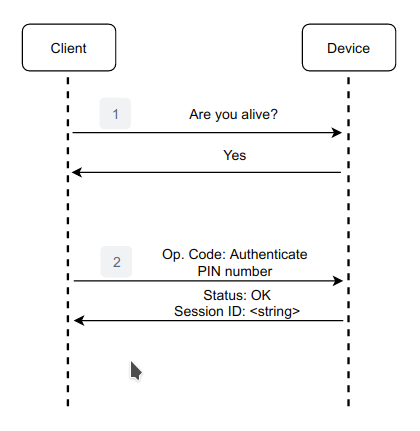
\includegraphics[width=0.5\textwidth]{./Images/authentication.png}
	\caption{Authentication Protocol}
	\label{fig:protocol:authentication}
\end{figure}

Before executing any operation the user must authenticate himself to the device.
Figure~\ref{fig:protocol:authentication} depicts the authentication protocol.
The user initiates by sending a message to check if the device is alive and connected to the computer. After the device responds with an acknowledge, the user software sends the authentication \ac{PIN}. The device will respond with a status parameter indicating failure or success. When it is successful, the session will be unlocked, allowing the user access to the main operations.

% -----------------------------------------------------
\subsection{Administration Protocol}\label{chap:solution:protocol:admin}
\begin{figure}[h]
	\centering
	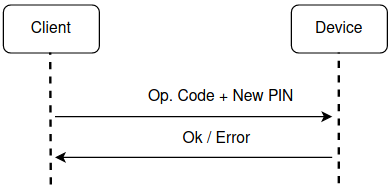
\includegraphics[width=0.5\textwidth]{./Images/change-PIN.png}
	\caption{Protocol to Change Authentication PIN}
	\label{fig:protocol:change-PIN}
\end{figure}

There is only one administration operation, changing the authentication \ac{PIN}, pictured in figure~\ref{fig:protocol:change-PIN}.
The user initiates by sending the change \ac{PIN} operation code, and the new \ac{PIN} number. The device responds with the return status of the operation.

% -----------------------------------------------------
\subsection{Secure Communications Protocol}\label{chap:solution:protocol:comms}

The protocol for operations which secure communications will be defined here. It covers the encryption and authentication operation, which enables secure communications and non-repudiation through qualified digital signatures.

%% Insert protocol image here
\begin{figure}[h]
	\centering
	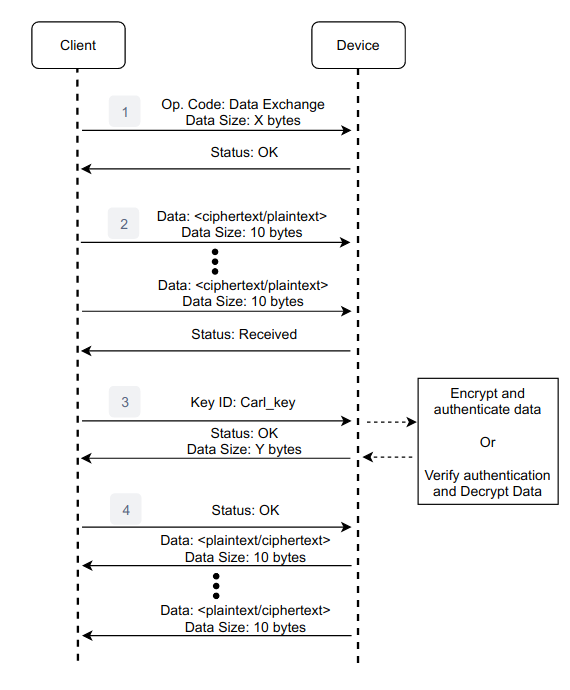
\includegraphics[width=0.6\textwidth]{./Images/data-exchange.png}
	\caption{Encryption+Authentication Protocol}
	\label{fig:protocol:data-exchange}
\end{figure}

The protocol to encrypt and authenticate data illustrated in figure~\ref{fig:protocol:data-exchange} consists of four phases:
It starts with the user sending the operation code and the data size. The box will respond with an OK message signaling the client application can begin to transmit the data. A maximum of X bytes per message can be transmitted. Each message contains a part of the data and the size of the data in that packet. When the transmission ends, the device confirms its reception.
In the third phase, the client software sends the ID of the symmetric key used to encrypt and authenticate communications with. The box will execute the cryptographic operations and return a status message and the encrypted data size.
When the client acknowledges its reception, the encrypted data with the \ac{MAC} and \ac{IV} parameters appended, will be sent back, one message at a time.

The protocol to decrypt and verify data authentication is very similar to the previous one, and is also pictured in figure~\ref{fig:protocol:data-exchange}. The differences are in phase three, after the ciphertext and symmetric key ID are transmitted, the device will decrypt and authenticate the data. It returns the operation status and the decrypted plaintext size if it was successful. It ends by transmitting the plaintext in the fourth phase to the client software.

\hfill
\hfill
%% ------------
\begin{figure}
	\centering     %%% not \center
	\subfigure[Generation Protocol]{\label{fig:protocol:signature-generate}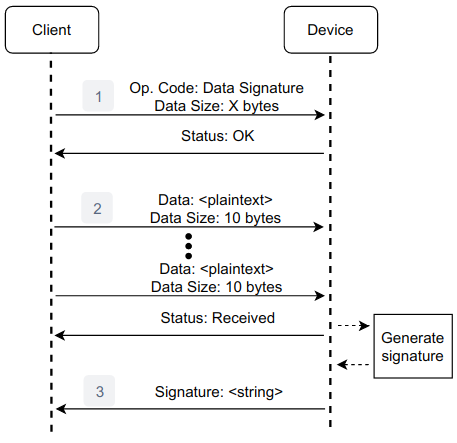
\includegraphics[width=79mm]{Images/signature-generate.png}}
	\subfigure[Verification Protocol]{\label{fig:protocol:signature-verify}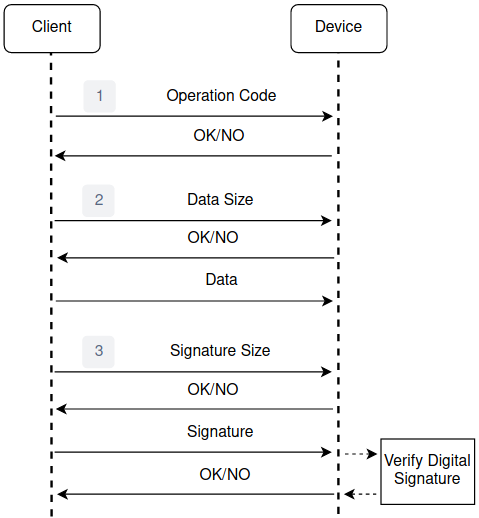
\includegraphics[width=79mm]{Images/signature-verify.png}}
	\caption{Digital Signature Generation Protocols}
\end{figure}

The next protocols are relating to the generation and verification of digital signatures.
The designed protocol for generation is represented in figure~\ref{fig:protocol:signature-generate}.
The user initiates by sending the operation code and the plaintext data size.
When the box responds with an OK message, the user transmits the data to be signed, one message at a time.
In possession of the data, the device will generate the digital signature using the device's private key. When finished the signature is sent back to the user.

The protocol for verifying digital signatures is pictured in figure~\ref{fig:protocol:signature-verify}.
After the user sends the operation code, and the box responds with an OK message, the user transmits the data, used by the signer to generate the signature, one message at a time.
When done, the user also sends the signature and the name of the signer, so the device knows what public key to use to verify the signature.
Then, the device will verify the digital signature using the signer's public key, the data and the signature. The result will be sent back to the user.

% -----------------------------------------------------
\subsection{Communication Management Protocol}\label{chap:solution:protocol:key}

The protocols for the communication management operations are detailed next. The operations are importation of public keys from the list provided to entities, generation of new symmetric keys and storage of newly received symmetric keys.

%% Insert protocol image here
\begin{figure}[h]
	\centering
	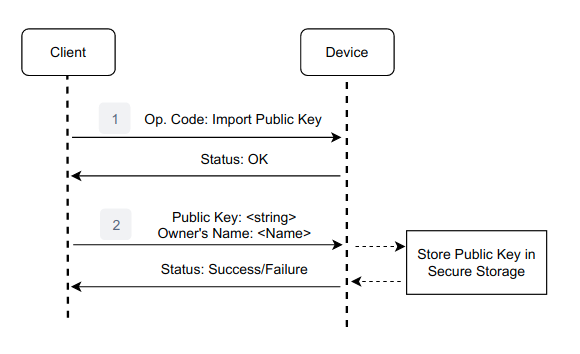
\includegraphics[width=0.5\textwidth]{./Images/import-pub-key.png}
	\caption{Import Public Key}\label{fig:protocol:import-pub}
\end{figure}

The protocol to import public keys is pictured in figure~\ref{fig:protocol:import-pub}.
Like previous protocols, it starts with the user sending a message with the operation code, indicating he wants to import someone's public key.
After the device responds with an OK signal, the user sends the public key, and the name of the public key's owner.
The device stores the key, associated to the owner's name, and informs the client software of the operation's success or failure.

\hfill
\hfill

%% -------------------------------------
Just like digital signatures, entities can share symmetric keys between each other if they each others public keys are stored in their devices. If not, they must first import them into their respective devices.

%% --------------------------
\begin{figure}
	\centering     %%% not \center
	\subfigure[Generate key]{\label{fig:protocol:new-key}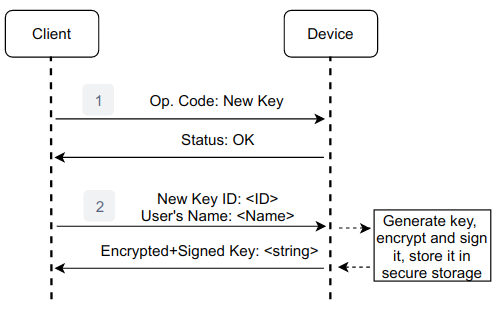
\includegraphics[width=79mm]{./Images/new-key.png}}
	\subfigure[Save key]{\label{fig:protocol:save-key}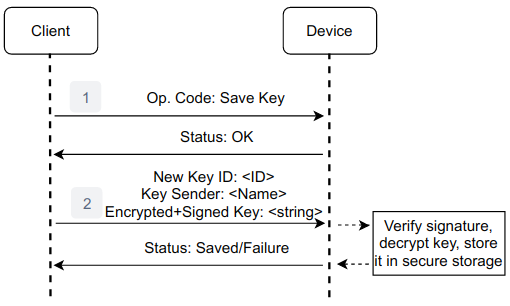
\includegraphics[width=79mm]{./Images/save-key.png}}
	\caption{Protocols for sharing keys}
\end{figure}

The protocol to generate a new symmetric key, and secure it to be shared with other entities is detailed in figure~\ref{fig:protocol:new-key}.
After both sides trade the operation code and OK status, the user sends the key ID, which will identify the symmetric key, and the name of the entity it will be shared with, so the device knows which public key to use to secure the key.
A new symmetric key will be generated and saved in the device's secure storage, with the key ID sent by the client application. The device encrypts and signs the key with public-key cryptography, and sends it back to the application, one message at a time. The user can then securely share the key with the other entity.

The protocol for the other user to save the newly received symmetric key, and store it inside their device is in figure~\ref{fig:protocol:save-key}.
After the operations code is sent and the OK signal is returned, the user sends the key ID, the name of the key sender, and the encrypted and signed key.
Then, the device verifies the signature and decrypts the key, subsequently saving it in the device's secure storage along with other symmetric keys already present.
